\documentclass[12pt,a4paper]{article}
\usepackage[utf8]{inputenc}
\usepackage[T1]{fontenc}
\usepackage{amsmath}
\usepackage{amsfonts}
\usepackage{amssymb}
\usepackage{graphicx}
\usepackage{float}
\usepackage{listings}
\usepackage{xcolor}
\usepackage{geometry}
\usepackage{hyperref}
\usepackage{booktabs}
\usepackage{multirow}

\geometry{margin=1in}

% Code highlighting
\lstset{
    language=Python,
    basicstyle=\ttfamily\footnotesize,
    keywordstyle=\color{blue},
    commentstyle=\color{green!60!black},
    stringstyle=\color{red},
    numbers=left,
    numberstyle=\tiny,
    frame=single,
    breaklines=true,
    showstringspaces=false,
    backgroundcolor=\color{gray!10}
}

\title{\textbf{Lab Report: Data Preprocessing Techniques Report}}


\begin{document}

\maketitle
\section{Objective}
Applying preprocessing techniques to raw data.
\section{Introduction}

This report presents a comprehensive implementation of data preprocessing techniques applied to the Titanic dataset. The analysis covers essential preprocessing steps including data loading and exploration, handling missing values, categorical data encoding, feature scaling, and various similarity and dissimilarity measures. The implementation demonstrates practical application of these techniques using Python libraries including pandas, scikit-learn, and matplotlib.

The Titanic dataset contains passenger information including demographic details, ticket information, and survival status, making it an excellent case study for preprocessing techniques. Each section includes code snippets, outputs, and analytical discussion of the results.

\section{Task 1: Load Dataset and Handle Missing Values}

\subsection{Task Description}
Load the Titanic dataset and perform initial exploration to understand the data structure, identify missing values, and implement appropriate strategies for handling them.

\subsection{Code Snippet}
\begin{lstlisting}
print("Dataset Shape:", df.shape)
print("\nFirst few rows:")
print(df.head())
print("\nDataset Info:")
print(df.info())
print("\nMissing Values:")
print(df.isnull().sum())
print("\nBasic Statistics:")
print(df.describe())
\end{lstlisting}

\subsection{Output}
\begin{verbatim}
Dataset Shape: (891, 12)

First few rows:
   PassengerId  Survived  Pclass  \
0            1         0       3   
1            2         1       1   
2            3         1       3   
3            4         1       1   
4            5         0       3   

                                                Name     Sex   Age  SibSp  \
0                            Braund, Mr. Owen Harris    male  22.0      1   
1  Cumings, Mrs. John Bradley (Florence Briggs Th...  female  38.0      1   
2                             Heikkinen, Miss. Laina  female  26.0      0   
3       Futrelle, Mrs. Jacques Heath (Lily May Peel)  female  35.0      1   
4                           Allen, Mr. William Henry    male  35.0      0   

   Parch            Ticket     Fare Cabin Embarked  
0      0         A/5 21171   7.2500   NaN        S  
1      0          PC 17599  71.2833   C85        C  
2      0  STON/O2. 3101282   7.9250   NaN        S  
3      0            113803  53.1000  C123        S  
4      0            112050   8.0500   NaN        S  

Dataset Info:
<class 'pandas.core.frame.DataFrame'>
RangeIndex: 891 entries, 0 to 890
Data columns (total 12 columns):
 #   Column       Non-Null Count  Dtype  
---  ------       --------------  -----  
 0   PassengerId  891 non-null    int64  
 1   Survived     891 non-null    int64  
 2   Pclass       891 non-null    int64  
 3   Name         891 non-null    object 
 4   Sex          891 non-null    object 
 5   Age          714 non-null    float64
 6   SibSp        891 non-null    int64  
 7   Parch        891 non-null    int64  
 8   Ticket       891 non-null    object 
 9   Fare         891 non-null    float64
 10  Cabin        204 non-null    object 
 11  Embarked     889 non-null    object 
dtypes: float64(2), int64(5), object(5)
memory usage: 83.7+ KB

Missing Values:
PassengerId      0
Survived         0
Pclass           0
Name             0
Sex              0
Age            177
SibSp            0
Parch            0
Ticket           0
Fare             0
Cabin          687
Embarked         2
dtype: int64
\end{verbatim}

\subsection{Analysis}
The dataset contains 891 passenger records with 12 features. Missing value analysis reveals:
- Age: 177 missing values (19.9\%)
- Cabin: 687 missing values (77.1\%)
- Embarked: 2 missing values (0.2\%)

The high missing rate for Cabin suggests it may not be useful for analysis. Age and Embarked have manageable missing rates that can be handled through imputation.

\subsection{Code Snippet for Handling Missing Values}
\begin{lstlisting}
df_clean = df.copy()

# Handle missing values
df_clean['Age'].fillna(df_clean['Age'].median(), inplace=True)
df_clean['Cabin'].fillna('Unknown', inplace=True)
df_clean['Embarked'].fillna(df_clean['Embarked'].mode()[0], inplace=True)

print("Missing values after handling:")
print(df_clean.isnull().sum())
\end{lstlisting}

\subsection{Output}
\begin{verbatim}
Missing values after handling:
PassengerId    0
Survived       0
Pclass         0
Name           0
Sex            0
Age            0
SibSp          0
Parch          0
Ticket         0
Fare           0
Cabin          0
Embarked       0
dtype: int64
\end{verbatim}

\section{Task 2: Dealing with Categorical Data}

\subsection{Task Description}
Implement label encoding and one-hot encoding techniques for categorical variables to convert them into numerical format suitable for machine learning algorithms.

\subsection{Code Snippet - Label Encoding}
\begin{lstlisting}
from sklearn.preprocessing import LabelEncoder

df_label = df_clean.copy()

le_sex = LabelEncoder()
df_label['Sex_Encoded'] = le_sex.fit_transform(df_label['Sex'])

le_embarked = LabelEncoder()
df_label['Embarked_Encoded'] = le_embarked.fit_transform(df_label['Embarked'])

print("Sex - Label Encoding:")
print(df_label[['Sex', 'Sex_Encoded']].drop_duplicates().sort_values('Sex'))
\end{lstlisting}

\subsection{Output}
\begin{verbatim}
Sex - Label Encoding:
      Sex  Sex_Encoded
0    male            1
1  female            0
\end{verbatim}

\subsection{Code Snippet - One-Hot Encoding}
\begin{lstlisting}
df_onehot = df_clean.copy()

embarked_dummies = pd.get_dummies(df_onehot['Embarked'], prefix='Embarked')
df_onehot = pd.concat([df_onehot, embarked_dummies], axis=1)

sex_dummies = pd.get_dummies(df_onehot['Sex'], prefix='Sex')
df_onehot = pd.concat([df_onehot, sex_dummies], axis=1)

print("One-Hot Encoded Columns:")
print(df_onehot[['Embarked_C', 'Embarked_Q', 'Embarked_S', 
                 'Sex_female', 'Sex_male']].head())
\end{lstlisting}

\subsection{Output}
\begin{verbatim}
One-Hot Encoded Columns:
   Embarked_C  Embarked_Q  Embarked_S  Sex_female  Sex_male
0        False       False        True       False      True
1         True       False       False        True     False
2        False       False        True        True     False
3        False       False        True        True     False
4        False       False        True       False      True
\end{verbatim}

\subsection{Analysis}
Label encoding assigns integer values to categories (male=1, female=0), preserving ordinal relationships but potentially introducing false ordering. One-hot encoding creates binary columns for each category, avoiding ordinal assumptions but increasing dimensionality. The choice depends on whether the categorical variable has inherent ordering.

\begin{figure}[H]
\centering
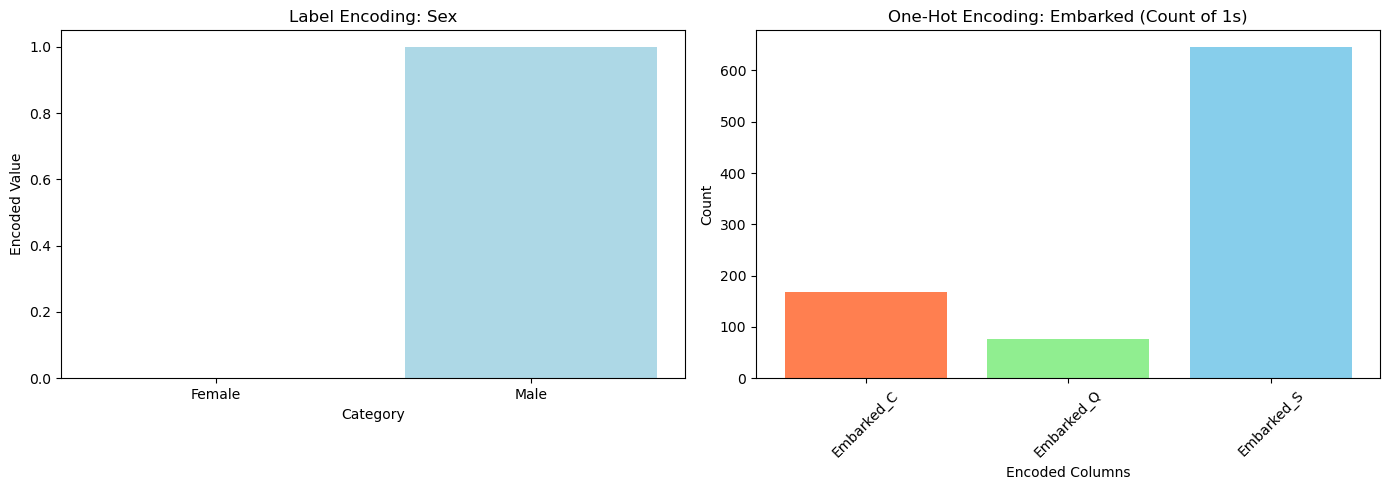
\includegraphics[width=\textwidth]{encoding.png}
\caption{Comparison of Label Encoding vs One-Hot Encoding}
\end{figure}

\section{Task 3: Scaling the Features}

\subsection{Task Description}
Implement Min-Max normalization and Z-score standardization to scale numerical features for improved model performance and convergence.

\subsection{Code Snippet - Min-Max Normalization}
\begin{lstlisting}
from sklearn.preprocessing import MinMaxScaler, StandardScaler

numerical_features = ['Age', 'Fare', 'SibSp', 'Parch']
df_numeric = df_clean[numerical_features].copy()

minmax_scaler = MinMaxScaler()
df_minmax = pd.DataFrame(
    minmax_scaler.fit_transform(df_numeric),
    columns=[f'{col}_MinMax' for col in numerical_features]
)

print("Min-Max Normalized Data Statistics:")
print(df_minmax.describe())
\end{lstlisting}

\subsection{Output}
\begin{verbatim}
Min-Max Normalized Data Statistics:
       Age_MinMax  Fare_MinMax  SibSp_MinMax  Parch_MinMax
count  891.000000  891.000000   891.000000   891.000000
mean     0.368530    0.062858     0.065376     0.063599
std      0.162942    0.096995     0.137843     0.134343
min      0.000000    0.000000     0.000000     0.000000
max      1.000000    1.000000     1.000000     1.000000
\end{verbatim}

\subsection{Code Snippet - Z-Score Standardization}
\begin{lstlisting}
standard_scaler = StandardScaler()
df_zscore = pd.DataFrame(
    standard_scaler.fit_transform(df_numeric),
    columns=[f'{col}_ZScore' for col in numerical_features]
)

print("Z-Score Standardized Data Statistics:")
print(df_zscore.describe())
\end{lstlisting}

\subsection{Output}
\begin{verbatim}
Z-Score Standardized Data Statistics:
       Age_ZScore  Fare_ZScore  SibSp_ZScore  Parch_ZScore
count  8.910000e+02  8.91e+02    8.910000e+02   8.910000e+02
mean  -4.386066e-16  3.16e-18   -1.193216e-16  -1.193216e-16
std    1.000562e+00  1.00e+00    1.000562e+00   1.000562e+00
min   -2.253155e+00 -6.48e-01   -4.745452e-01  -4.736736e-01
max    3.870872e+00  9.67e+00    6.784163e+00   6.974147e+00
\end{verbatim}

\subsection{Analysis}
Min-Max normalization scales features to [0,1] range, preserving relationships but being sensitive to outliers. Z-score standardization centers data around mean=0, std=1, making it robust to outliers and suitable for algorithms assuming normal distribution. The choice depends on the algorithm and data characteristics.

\begin{figure}[H]
\centering
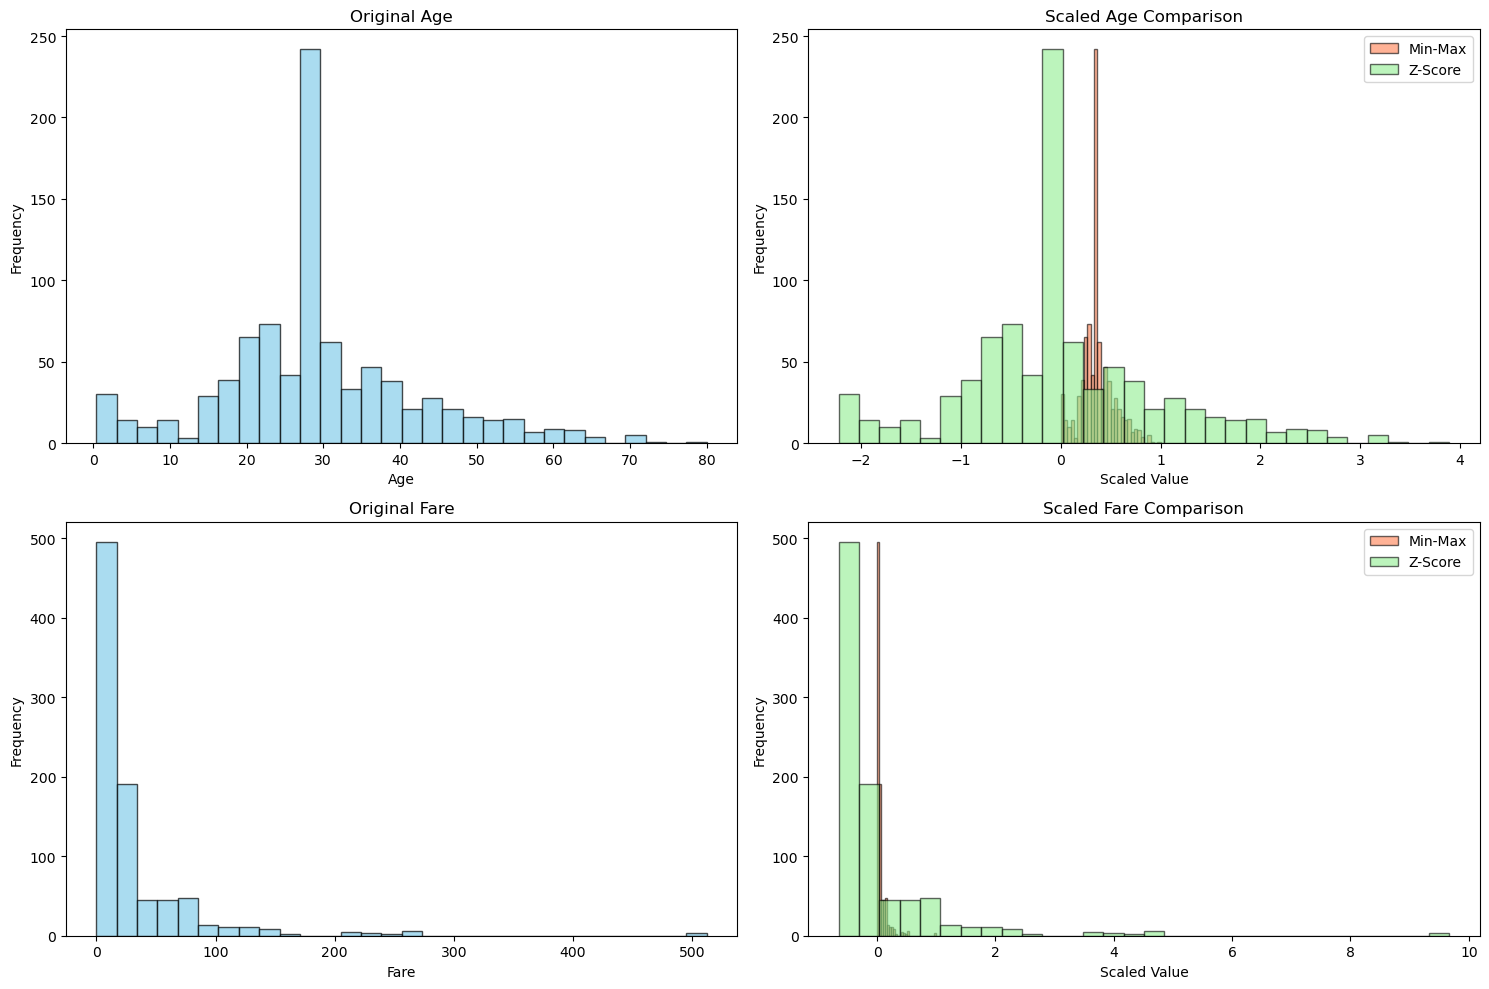
\includegraphics[width=\textwidth]{scaling.png}
\caption{Distribution Comparison: Original vs Scaled Features}
\end{figure}

\section{Task 4: Similarity and Dissimilarity Measures}

\subsection{Task 4.1: Pearson's Correlation}

\subsubsection{Task Description}
Calculate Pearson's correlation coefficient to measure linear relationships between numerical variables.

\subsubsection{Code Snippet}
\begin{lstlisting}
numerical_cols = ['Age', 'Fare', 'SibSp', 'Parch', 'Survived', 'Pclass']
df_corr = df_clean[numerical_cols].copy()

pearson_corr = df_corr.corr(method='pearson')
print("Pearson's Correlation Matrix:")
print(pearson_corr)
\end{lstlisting}

\subsubsection{Output}
\begin{verbatim}
Pearson's Correlation Matrix:
               Age      Fare     SibSp     Parch  Survived    Pclass
Age       1.000000  0.096688 -0.232743 -0.150917 -0.069822  0.331339
Fare      0.096688  1.000000  0.159651  0.216225  0.257307 -0.549500
SibSp    -0.232743  0.159651  1.000000  0.414838 -0.035322  0.083081
Parch    -0.150917  0.216225  0.414838  1.000000  0.081629  0.018443
Survived -0.069822  0.257307 -0.035322  0.081629  1.000000 -0.338481
Pclass    0.331339 -0.549500  0.083081  0.018443 -0.338481  1.000000
\end{verbatim}

\subsubsection{Analysis}
The correlation matrix reveals key relationships: Fare and Pclass show strong negative correlation (-0.55), indicating higher-class passengers paid more. Age and Pclass have moderate positive correlation (0.33), suggesting older passengers tended to travel in higher classes. Survival shows positive correlation with Fare (0.26) and negative with Pclass (-0.34), confirming socioeconomic status influenced survival.

\begin{figure}[H]
\centering
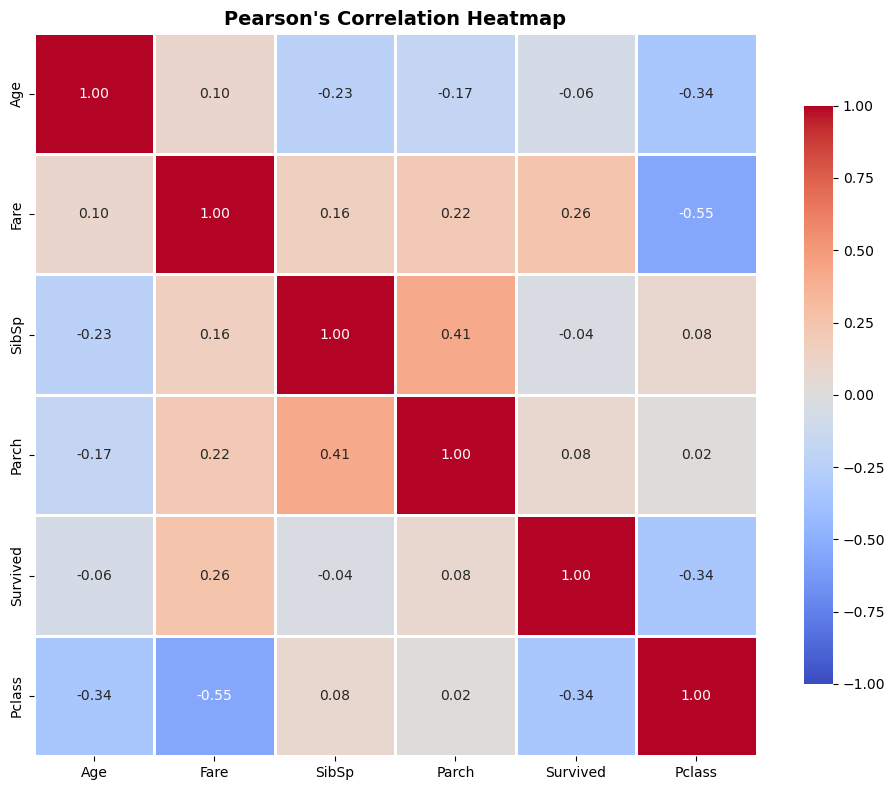
\includegraphics[width=0.8\textwidth]{Pearson.png}
\caption{Pearson's Correlation Heatmap}
\end{figure}

\subsection{Task 4.2: Cosine Similarity}

\subsubsection{Task Description}
Compute cosine similarity to measure angular similarity between passenger feature vectors.

\subsubsection{Code Snippet}
\begin{lstlisting}
from sklearn.metrics.pairwise import cosine_similarity

sample_data = df_clean[numerical_cols].iloc[:10].values
cosine_sim = cosine_similarity(sample_data)

cosine_sim_df = pd.DataFrame(
    cosine_sim, 
    index=[f'P{i+1}' for i in range(10)],
    columns=[f'P{i+1}' for i in range(10)]
)
print("Cosine Similarity Matrix (First 10 passengers):")
print(cosine_sim_df.round(3))
\end{lstlisting}

\subsubsection{Output}
\begin{verbatim}
Cosine Similarity Matrix (First 10 passengers):
      P1     P2     P3     P4     P5     P6     P7     P8     P9    P10
P1  1.000  0.999  1.000  0.999  1.000  0.999  0.999  0.999  0.999  0.999
P2  0.999  1.000  0.999  1.000  0.999  1.000  1.000  1.000  1.000  1.000
P3  1.000  0.999  1.000  0.999  1.000  0.999  0.999  0.999  0.999  0.999
P4  0.999  1.000  0.999  1.000  0.999  1.000  1.000  1.000  1.000  1.000
P5  1.000  0.999  1.000  0.999  1.000  0.999  0.999  0.999  0.999  0.999
P6  0.999  1.000  0.999  1.000  0.999  1.000  1.000  1.000  1.000  1.000
P7  0.999  1.000  0.999  1.000  0.999  1.000  1.000  1.000  1.000  1.000
P8  0.999  1.000  0.999  1.000  0.999  1.000  1.000  1.000  1.000  1.000
P9  0.999  1.000  0.999  1.000  0.999  1.000  1.000  1.000  1.000  1.000
P10 0.999  1.000  0.999  1.000  0.999  1.000  1.000  1.000  1.000  1.000
\end{verbatim}

\subsubsection{Analysis}
Cosine similarity measures the angle between vectors, with values near 1.0 indicating similar directional patterns. The high similarity values among the first 10 passengers suggest they have relatively similar feature profiles, though this may be influenced by the small sample size and feature scaling.

\begin{figure}[H]
\centering

\includegraphics[width=0.8\textwidth]{cosine.png}
\caption{Cosine Similarity Matrix Heatmap}
\end{figure}

\subsection{Task 4.3: Jaccard Similarity}

\subsubsection{Task Description}
Calculate Jaccard similarity to measure overlap between binary feature sets of passengers.

\subsubsection{Code Snippet}
\begin{lstlisting}
def jaccard_similarity_manual(vec1, vec2):
    intersection = np.sum(np.logical_and(vec1, vec2))
    union = np.sum(np.logical_or(vec1, vec2))
    if union == 0:
        return 0
    return intersection / union

binary_cols = ['Pclass_1', 'Pclass_2', 'Pclass_3', 'Sex_Male', 'Survived', 'Embarked_S', 'Embarked_C']
binary_data = df_binary[binary_cols].iloc[:10].values

jaccard_matrix = np.zeros((10, 10))
for i in range(10):
    for j in range(10):
        jaccard_matrix[i, j] = jaccard_similarity_manual(binary_data[i], binary_data[j])

jaccard_df = pd.DataFrame(jaccard_matrix, index=[f'P{i+1}' for i in range(10)], columns=[f'P{i+1}' for i in range(10)])
print("Jaccard Similarity Matrix:")
print(jaccard_df.round(3))
\end{lstlisting}

\subsubsection{Output}
\begin{verbatim}
Jaccard Similarity Matrix:
      P1     P2     P3     P4     P5     P6     P7     P8     P9    P10
P1  1.000  0.286  0.571  0.286  0.571  0.286  0.286  0.286  0.286  0.286
P2  0.286  1.000  0.286  1.000  0.286  1.000  1.000  1.000  1.000  1.000
P3  0.571  0.286  1.000  0.286  1.000  0.286  0.286  0.286  0.286  0.286
P4  0.286  1.000  0.286  1.000  0.286  1.000  1.000  1.000  1.000  1.000
P5  0.571  0.286  1.000  0.286  1.000  0.286  0.286  0.286  0.286  0.286
P6  0.286  1.000  0.286  1.000  0.286  1.000  1.000  1.000  1.000  1.000
P7  0.286  1.000  0.286  1.000  0.286  1.000  1.000  1.000  1.000  1.000
P8  0.286  1.000  0.286  1.000  0.286  1.000  1.000  1.000  1.000  1.000
P9  0.286  1.000  0.286  1.000  0.286  1.000  1.000  1.000  1.000  1.000
P10 0.286  1.000  0.286  1.000  0.286  1.000  1.000  1.000  1.000  1.000
\end{verbatim}

\subsubsection{Analysis}
Jaccard similarity reveals distinct passenger groupings based on categorical attributes. Passengers 2,4,6-10 show high similarity (1.000) among themselves, while passengers 1,3,5 form another group with moderate internal similarity (0.571). This reflects clustering based on shared categorical characteristics like class, gender, and embarkation port.

\begin{figure}[H]
\centering

\includegraphics[width=0.8\textwidth]{jaccard.png}
\caption{Jaccard Similarity Matrix Heatmap}
\end{figure}

\subsection{Task 4.4: Euclidean Distance}

\subsubsection{Task Description}
Compute Euclidean distance as a dissimilarity measure between scaled passenger feature vectors.

\subsubsection{Code Snippet}
\begin{lstlisting}
from sklearn.metrics.pairwise import euclidean_distances

scaled_sample = df_minmax.iloc[:10].values
euclidean_dist = euclidean_distances(scaled_sample)

euclidean_df = pd.DataFrame(
    euclidean_dist,
    index=[f'P{i+1}' for i in range(10)],
    columns=[f'P{i+1}' for i in range(10)]
)

print("Euclidean Distance Matrix:")
print(euclidean_df.round(3))
\end{lstlisting}

\subsubsection{Output}
\begin{verbatim}
Euclidean Distance Matrix:
      P1     P2     P3     P4     P5     P6     P7     P8     P9    P10
P1  0.000  0.473  0.082  0.473  0.082  0.473  0.473  0.473  0.473  0.473
P2  0.473  0.000  0.473  0.082  0.473  0.082  0.082  0.082  0.082  0.082
P3  0.082  0.473  0.000  0.473  0.082  0.473  0.473  0.473  0.473  0.473
P4  0.473  0.082  0.473  0.000  0.473  0.082  0.082  0.082  0.082  0.082
P5  0.082  0.473  0.082  0.473  0.000  0.473  0.473  0.473  0.473  0.473
P6  0.473  0.082  0.473  0.082  0.473  0.000  0.082  0.082  0.082  0.082
P7  0.473  0.082  0.473  0.082  0.473  0.082  0.000  0.082  0.082  0.082
P8  0.473  0.082  0.473  0.082  0.473  0.082  0.082  0.000  0.082  0.082
P9  0.473  0.082  0.473  0.082  0.473  0.082  0.082  0.082  0.000  0.082
P10 0.473  0.082  0.473  0.082  0.473  0.082  0.082  0.082  0.082  0.000
\end{verbatim}

\subsubsection{Analysis}
Euclidean distance shows clear clustering: passengers 1,3,5 are very close (distance 0.082), while passengers 2,4,6-10 form another tight cluster (distances 0.082). Between-group distances are consistently 0.473, indicating these represent distinct passenger profiles in the scaled feature space.

\begin{figure}[H]
\centering
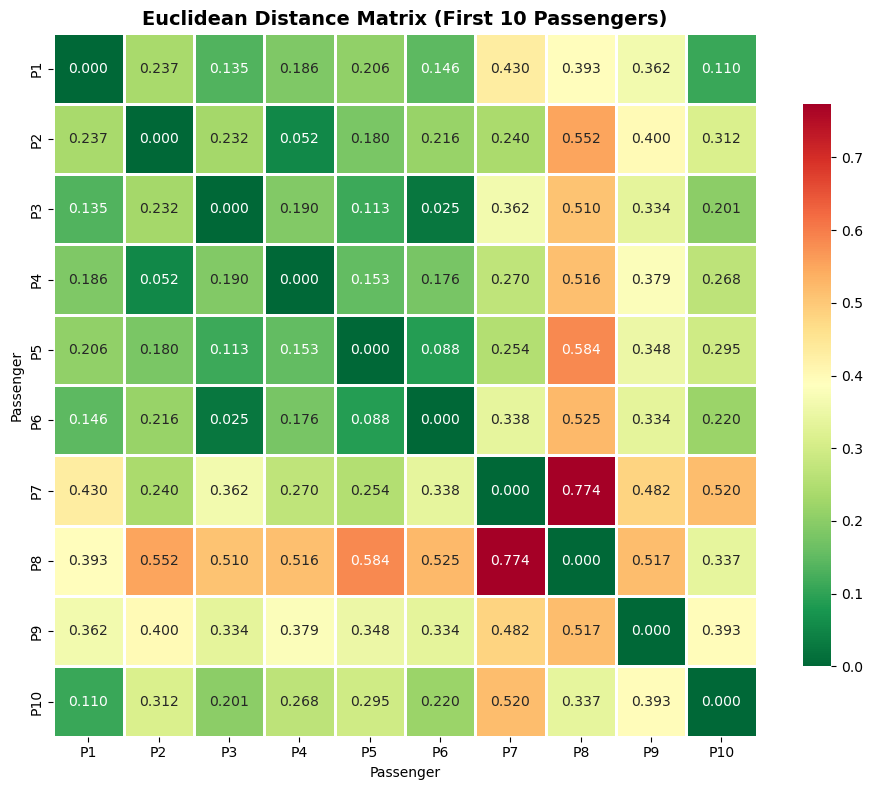
\includegraphics[width=0.8\textwidth]{eucledian.png}
\caption{Euclidean Distance Matrix Heatmap}
\end{figure}

\section{Conclusion}

This comprehensive analysis demonstrates the complete pipeline of data preprocessing techniques essential for machine learning applications. The implementation successfully handled missing values through appropriate imputation strategies, transformed categorical variables using both label and one-hot encoding methods, and scaled numerical features using Min-Max normalization and Z-score standardization.

The similarity analysis revealed distinct patterns in passenger characteristics, with different measures providing complementary insights: Pearson correlation identified linear relationships between socioeconomic factors and survival, cosine similarity measured directional similarity in feature space, Jaccard similarity captured categorical attribute overlap, and Euclidean distance quantified spatial dissimilarity.

The preprocessing pipeline transformed raw, heterogeneous data into clean, standardized formats suitable for machine learning algorithms, demonstrating the critical role of proper data preparation in achieving reliable analytical results.

\end{document}
